\chapter{\protect\textsc{Carico}}
% This chapter may be called something else\ldots but in general the
% idea is that you have one (or a few) ``meat'' chapters which describe
% the work you did in technical detail.
% \begin{tcolorbox}[boxsep=0mm,left=2.5mm,right=2.5mm]
    % \textbf{Design and Implementation:} {\em In this section, I will outline the
    % goals of my system. I will give a brief overview of the chapter structure,
    % summarising each core section and what I achieve.}
% \end{tcolorbox}
This chapter details \textsc{Carico}, a federated, asynchronous,
memory-limited algorithm, building upon the principles of \textsc{Pronto}.
\textsc{Carico} differentiates itself from \textsc{Pronto} for the following
reasons:
\begin{enumerate}
    \item Rather than performing standard FPCA, \textsc{Carico} applies FSVD on
        observed [0,1]-normalised resource usage. Subsequently, \textsc{Carico} uses
        new interpretations for the results of SVD and modifies the
        Subspace-Merge to preserve the interpretations.
    \item \textsc{Carico} presents a novel continuous and \textbf{comparable}
        capacity signal function that combines the new model interpretations
        with a Node's current resource usage to calculate its estimated
        workload capacity.
    \item \textsc{Carico} makes two assumptions to translate the calculated
        capacity signal into a signal that is both \textbf{reservable} and uses
        the number of Pods as its unit of measure.
\end{enumerate}
As this algorithm produces a signal that measures "capacity", I will refer to it
as \textsc{Carico} - "load" in Italian.

\section{Capacity Signal}
In Section \ref{sec:intro-weakness}, we identified critical limitations of
\textsc{Pronto}'s binary ``Reject-Job" signal within the Kubernetes ecosystem:
its lack of comparable Node scoring and inability to handle Pod start-up
latencies. While one could conceivably compare the number of detected spikes,
it's difficult to quantitatively assign or reserve ``peak detections" for
incoming Pods. Furthermore, as shown in Figure
\ref{fig:podcount-util-pressure}, contention metrics often do not change
proportionally to the number of tasks assigned, making them difficult to
reserve accurately.

These limitations demand a signal reflecting varying levels of contention
and offering a predictable, scalar relationship with task assignments.
\texttt{kube-schedulers}'s reservation of a Node's resource highlights the
potential use of a capacity metric. FPCA's interpretations focus on the
variability within telemetry data rather than its absolute value, and therefore,
is not suitable for calculating measures of capacity. The subsequent
challenge was to find a means of transforming \textsc{Pronto}'s mathematical
framework to produce values that could be interpreted as the direction and
magnitude of recent workload's resource usage. Only once we had this
interpretation, could we then develop a continuous, comparable, and reservable
signal that could effectively and accurately guide scheduling decisions.

\section{Local Model}
\label{sec:local-model-construction}
\textsc{Carico} assumes a batch of telemetric data $\mathbf{A}$ is an $m \times
n$ matrix, where $\mathbf{A}$ contains $n$ samples of $m$-dimensional columns of
data. Each dimension in the vector represents a different resource, where the
value $0$ indicates that full capacity is available for that resource and $1$
indicates that the resource is being fully used ([0,1]-normalised). As we
are no longer mean-centering the dataset before applying SVD, \textbf{PCA's
interpretations no longer apply to the resulting $\mathbf{U}$ and $\Sigma$
matrices}.

Instead, \textsc{Carico} is built on top of  a different set of interpretations.
Using the Lemma proved in Appendix \ref{app:vector-to-avg}, we can interpret the
first left singular vector $u_1$ in $\mathbf{U}$ as a pseudo-weighted average
direction of the datapoints in the matrix: ``larger" or more aligned columns
contribute more significantly to the sum defining $u_1$, and thus to its final
direction. Thus $u_1$ behaves as a primary indicator of the direction of the
current workload's resource usage.

While knowing the proportion of resource usage is useful, it is also important
to be able to differentiate between lightweight workloads and more intense
workloads. For this, \textsc{Carico} uses the first singular value $\sigma_1$ in
$\Sigma$. Given $\sigma_1(\mathbf{A})$ and $u_1$ correspond to the first
singular value and first left singular vector of a batch of telemetry
$\mathbf{A}$:
\begin{align}
    \sigma_1(\mathbf{A})^2 &= u_1^T \mathbf{AA}^T u_1 \\
    &= (u_1^T \mathbf{A})^2
\end{align}
Given $a_j$ is the $j$-th column of $\mathbf{A}$, $\sigma_1(\mathbf{A})^2$ can be
interpreted as the sum of squared scalar projections of columns in $\mathbf{A}$:
$\sigma_1(\mathbf{A})^2 = \sum_{j=1}^n (u^T a_j)^2$.

Furthermore, the first singular value can be shown to scale with resource usage.
Given two batches of telemetry $\mathbf{A}$ and $\mathbf{B}$ where batch
$\mathbf{B}$ experienced more resource usage ($0 \leq a_{ij} \leq b_{ij} \leq 1$
for all $i,j$), it is shown in Appendix \ref{sec:app-monotonicity} that the
first singular value of $\mathbf{B}$ will be greater than or equal to that of
$\mathbf{A}$ ($\sigma_1(\mathbf{A}) \leq \sigma_1(\mathbf{B})$). Subsequently,
the first singular value makes a good indicator of measured resource usage.

\section{Subspace Merging}
\label{sec:local-merge}
While we have shown that the results from performing SVD on [0,1]-normalised
telemetry data can have useful interpretations, the resulting $\sigma_1$ can
grow with each Incremental-SVD (Appendix \ref{sec:app-concatenate}):\\
Given two non-negative matrices $\mathbf{A} \in \mathbb{R}^{m \times n_1}$ and
$\mathbf{B} \in \mathbb{R}^{m \times n_2}$, the first singular value of the
concatenated matrix $\mathbf{C} = [\mathbf{A}, \mathbf{B}]$ is greater than or
equal to the maximum of the first singular values of $\mathbf{A}$ and
$\mathbf{B}$:
\[ \sigma_1([\mathbf{A}, \mathbf{B}]) \geq \max(\sigma_1(\mathbf{A}),
\sigma_1(\mathbf{B})) \]

This property is important, as we established earlier that \textsc{Carico} uses
$\sigma_1$ as an indicator of the magnitude of resource usage. If $\sigma_1$ can
increase while the measured telemetry reports a stable magnitude of resource
usage, its interpretation no longer holds.

To solve this, \textsc{Carico} scales the concatenated matrices using non-negative scalar
weights $\gamma_{\mathbf{A}} = \sqrt{w_{\mathbf{A}}}$ and
$\gamma_{\mathbf{\mathbf{B}}} = \sqrt{w_{\mathbf{\mathbf{B}}}}$ such that
$w_{\mathbf{A}} + w_{\mathbf{\mathbf{B}}} = 1$. This method still preserves the
earlier interpretations:

\begin{itemize}
    \item \textbf{First Left Singular Vector:}\\
        The resulting first singular vector $u_1$ of the concatenated matrix $\mathbf{C} =
        [\gamma_{\mathbf{A}}\mathbf{A},
        \gamma_{\mathbf{\mathbf{B}}}\mathbf{\mathbf{B}}]$ still behaves as a
        pseudo-weighted average, but with the contributions of the input telemetry
        further weighted according to the scalar weights. Furthermore, the
        weights can be used as a forget factor similar to $\gamma$ in
        \textsc{Pronto}.
    \item \textbf{First Singular Value:}\\
        Appendix \ref{sec:app-scale} proves that the resulting first
        singular value $\sigma_1(\mathbf{C})$ and the first left singular vector
        $u_1$ of the concatenated matrix $\mathbf{C} =
        [\gamma_{\mathbf{A}}\mathbf{A}, \gamma_{\mathbf{B}}\mathbf{B}]$ have the
        following property:
        \[ \min(P_{\mathbf{A}}(u_1),P_{\mathbf{B}}(u_1))
        \leq \sigma_1(\mathbf{C})^2 \leq
        \max(P_{\mathbf{A}}(u_1),P_{\mathbf{B}}(u_1)) \]
        where $P_{\mathbf{M}}(u)$ is the sum of squared scalar projections of
        the columns in $\mathbf{M}$ onto $u$. As $\sigma_1(\mathbf{C})^2$ is a
        convex combination of $P_{\mathbf{A}}(u_1)$ and $P_{\mathbf{B}}(u_1)$,
        it is bound and acts as a weighted average of two projected sums in the
        new workload direction.
\end{itemize}

\section{Capacity Signal Function}
\label{sec:capacity-signal}
Using the established interpretations:
\begin{itemize}
    \item $u_1$: the pseudo-weighted average direction of resource usage of
        recent workloads
    \item $\sigma_1$: the magnitude of the resource usage of recent workloads
\end{itemize}
we can derive a new capacity signal that considers both the estimated
workload resource usage and its current resource usage. Given the the current
[0,1]-normalised resource usage vector for the node $y$, the first singular
value and left singular vector $\sigma_1$, $u_1$ from the latest subspace ($U$,
$\Sigma$), a Node's estimated ``Capacity" signal $k$ is given by:
\begin{align}
    y_{\text{predict}} = y + k * \sigma_1 u_1 \\
    \max_k \forall i: y_{\text{predict}} < 1
\end{align}
The resulting Capacity signal $k$ represents how many "units" of the learned
``average" workload ($\sigma_1 u_1$) can be added to the current workload ($y$)
before any single resource dimension hits its normalised capacity of 1.
% This calculation does
% ignore the fact that $\sigma_i^2$ is a sum of $n$ projected distances, where $n$
% is the number of samples. However, this will only matter if compute nodes use
% different batch sizes, otherwise, this $\frac{1}{\sqrt{n}}$ factor is absorbed
% into $k$.
%
\subsection{Example Scenarios}
\label{sec:signal-example-scenario}
To better understand how this signal works, I explore how the Capacity signal
changes under different different workloads. These scenarios will also be used to
verify the Capacity signal implementation in the prototype.

\begin{figure}[ht]
    \centering
    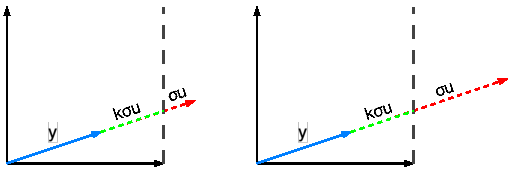
\includegraphics[width=\textwidth]{images/conflicting-workload.pdf}
    \caption{Visualisations of a Node's resource usage $y$ and expected resource
    usage $\sigma_1 u_1$ when learning of conflicting resource utilisation.}
    \label{fig:conflicting-workload}
\end{figure}

Figure \ref{fig:conflicting-workload} presents the scenario where a Node updates
its local model, learning that the experienced workload has increased in
resource usage ($\sigma_1$ has increased). This means that a smaller constant
$k$ is needed before the combined vectors cross a resource boundary. The Node,
thus, advertises a smaller capacity signal as it has less capacity for
the expected resource usage.

\begin{figure}[ht]
    \centering
    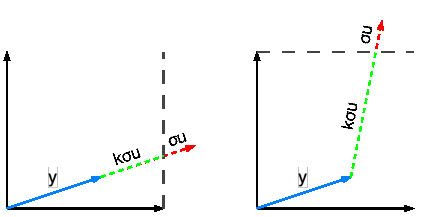
\includegraphics[width=0.8\textwidth]{images/complementary-workload.pdf}
    \caption{Visualisations of a Node's resource usage $y$ and expected resource
    usage $\sigma_1 u_1$ when learning of complementary resource utilisation.}
    \label{fig:complementary-workload}
\end{figure}

Figure \ref{fig:complementary-workload} presents the scenario where a Node updates
its local model, learning that the learned workload is using more resources but
in a different direction. This could be described as a complementary workload as
the the new expected resource utilisation requires a larger constant $k$ to
cross a resource boundary. Therefore, the Node advertises a higher capacity
signal as it has more capacity for the new expected resource utilisation.

\section{Reserve Cost and Capacity}
\label{sec:spazio-cost-capacity}
Like \textsc{Pronto}, \textsc{Carico}'s signal uses its current resource usage, and therefore, only
reflects Pods that have been scheduled and are running on the Node. For
\textsc{Carico} to account for Pod startup latency, the central scheduler must be able
to predict the a Pod's effect on a Node's signal. Consequently, \textsc{Carico}
assumes that Nodes know the number of currently running Pods and have the
ability to estimate their:
\begin{enumerate}
    \item \textbf{Baseline Capacity Signal:} the Capacity signal when no Pods
        are running
    \item \textbf{Per-Pod-Cost:} the estimated drop in Capacity signal will drop
        when a single Pod starts running.
\end{enumerate}
Section \ref{sec:estimating-cost} implements and compares different prediction
methods. With this information, a Node can calculate its Pod-Capacity (Capacity
given in units of Pods) from:
\begin{align}
    \text{Pod-Capacity} &= \frac{\text{Current Capacity Signal}}{\text{Per-Pod-Cost}} \\
    \text{Pod-Capacity} &= \frac{\text{Baseline Capacity Signal}}{\text{Per-Pod-Cost}}
    - \text{Current Pod Count}
\end{align}
This metric has two useful properties:
\begin{itemize}
    \item \textbf{Dual-Mode:} Pod-Capacity can be calculated
        using two equations. This is especially useful in Kubernetes as
        container creation and deletion can cause significant resource spikes,
        even with filtering in Figure \ref{fig:filtered-metrics-eval}, impacting
        immediate predictions.
        To combat this noise, Nodes can switch to predicting Pod-Capacity from
        previous Baseline and Per-Pod-Cost estimates. This reduces fluctuations
        in a Node's advertised Pod-Capacity and improves scheduling decisions
    \item \textbf{Unit of Measure:} As its unit of measure is in terms
        the number of Pods, it simplifies the central scheduler's logic,
        removing the need to keep track of each Node's Per-Pod-Cost.
\end{itemize}

\section{Central Scheduler}
Each Node $n$ will broadcast its $\text{Pod-Capacity}_n$ to a central scheduler. This
scheduler also tracks each Node's reserved amount as $\text{\# Pods Reserved}_n$. For
each Pending Pod, the scheduler performs the following operations:
\begin{itemize}
    \item \textbf{Filter:} Filters out all Nodes $n$ with $\text{Pod-Capacity}_n -
        \text{\# Pods Reserved}_n < 1$. Thus, the scheduler only considers Nodes
        with enough resources for another Pod. While reducing the threshold
        could pack more Pods on a Node, overallocation could result in OOM kills
        if there isn't enough memory available on a Node for all the Pods.
    \item \textbf{Score:} Score Nodes $n$ by $\text{Pod-Capacity}_n - \text{\#
        Pods Reserved}_n$. This ensures we allocate to Nodes which can fit more
        Pods.
    \item \textbf{Reserve:} Once a Node $n$ has been chosen, we increment
        $\text{\# Pods Reserved}_n$ by $1$. Once a scheduled Pod
        is no longer in the Pending state, the central scheduler decrements
        $\text{\# Pods Reserved}_n$ by $1$ for the Node $n$ the Pod was assigned
        to.
\end{itemize}

\section{Properties}
\textsc{Pronto} is designed to be \textit{federated, streaming} and
\textit{unsupervised}. \textsc{Carico} exhibits identical properties while also
considering the existence of communication and Pod start-up latency.

\textbf{Federated:}
While \textsc{Carico} uses a central scheduler to score Nodes and perform the final
Bind operation, it can still be considered federated because of its use
of FSVD: individual Nodes have a unified view of the global workload
while maintaining their individual autonomy to set their own score.

\textbf{Streaming:} Like \textsc{Pronto}, \textsc{Carico} only requires a single
pass over the incoming data in order to update its estimates. In addition,
Incremental-SVD only requires memory linear to the number of features
considered; given batches of dimension $d \times b$, the required memory is
proportional to $\mathcal{O}(d)$. This memory footprint can be further reduced
with low-rank approximation.

\textbf{Unsupervised:} \textsc{Carico} uses FSVD and assumptions about the
collected telemetry to generate values with capacity-based interpretations.
While this greatly differs from \textsc{Pronto} and its use of FPCA,
\textsc{Carico} still exploits the resulting subspace estimate along with the
incoming data to reveal patterns in recent resource-usage.

\textbf{Comparable:} \textsc{Pronto} is a binary signal, which makes it
difficult to score Nodes. \textsc{Carico}'s $\text{Pod-Capacity} \in
\mathbb{R}$, allowing Nodes to be filtered and scored against each other.

\textbf{Latency Resilient:} Unlike \textsc{Pronto} which assumes no communication
latency, \textsc{Carico} was designed with Kubernetes in mind, and thus must consider
possible latency in communication and Pod startup. \textsc{Carico}'s
$\text{Pod-Capacity}$'s unit of measure allows the central scheduler to easily
track the estimated cost of Pods in-flight, ensuring subsequent scheduling
decisions do not mistakenly overload a Node with a high $\text{Pod-Capacity}$.
%
% There are several methods to integrating the reserve cost into the signal to be
% sent to the central scheduler. The first method involves sending the signal and
% the reserve cost as separate values. On pod bind, we reserve the latest pod cost
% from the signal, and only relinquish the reserved amount once the central
% scheduler \verb|kube-apiserver| listener detects the pod is no longer Pending.
% This method requires the central scheduler to keep track of both the pods on
% each node and the pod-cost when the pod was bound.
%
% I instead chose to integrate the reserve quantity directly into the signal: each
% node calculates its available capacity in terms of no. of pods using two equations:
% \[ \text{avail. capacity from signal} = \frac{\text{signal}}{\text{per-pod-cost}} \\
   % \text{avail. capacity from no. of pods} = \frac{\text{capacity}}{\text{per-pod-cost}} -
   % \text{no. of pods} \]
%
% We use to functions for different situations. Typically, we calculate the
% available capacity from the latest signal measurements. However, if we detect a
% recent container event, the remote \verb|pronto| pod calculates the capacity
% from the pod count. This is to reduce the instability introduced by the
% container runtime. Furthermore, with this signal, the central scheduler does not
% have to record the per-pod-cost at bind time as the signal is now given in terms
% of individual pod counts. This simplifies the central scheduler and reduces the
% memory demand on.
%

\section{Related Work}
This section briefly identifies how \textsc{Carico} fits into the current
landscape of Kubernetes schedulers.

\subsection{Federated and Distributed Scheduling}
\textsc{Pronto} is described as a federated algorithm that executes plans in a
decentralised fashion. Each computing node makes independent decisions for task
assignments without needing global synchronisation. Custom Kubernetes schedulers
have been designed to extend the Kubernetes architectures with modular,
two-level, or distributed architectures \cite{beltre2019kubesphere, casquero2019distributed, luong2019multi, zhang2019multi}. However, the new
federated scheduler returns to a centralised architecture, mirroring the default
Kubernetes scheduler (\texttt{kube-scheduler}) with a single dispatcher on the
master node and has access to a global view of the Nodes.

\subsection{Performance-Aware and Predictive Scheduling}
As a performance-aware scheduler, \textsc{Carico} employs
dimensionality-reduction technique to efficiently process the vast amount of
telemetry data produced by each Node, with the goal of predicting a Node's
capacity for incoming workloads. While, CPU and RAM utilisation are common
metrics for performance-aware Kubernetes schedulers~\cite{bao2019deep,
beltre2019kubesphere, bestari2020dynamic, carvalho2021qoe, toka2021ultra},
\textsc{Carico} distinguishes itself with its ability to work with any metric
that can be [0,1]-normalised such that 0 indicates full capacity available and 1
indicates no capacity remaining.

Furthermore, the dynamic nature of Kubernetes workloads strongly suggest that
predictive techniques could improve scheduling efficiency and resource
utilisation, and still remains an open research
topic~\cite{carrion2022kubernetes}.

\subsection{Machine Learning-Based Schedulers}
Machine Learning (ML) algorithms  are increasingly adopted in scheduling to
learn from data and improving decision quality. These range from
Deep-Reinforcement learning-based schedulers \cite{bao2019deep, huang2020rlsk,
peng2021dl2, han2021tailored} that use reward functions to continuously improve
scheduling decisions, to domain-specifc to application or resource utilisation
predictions~\cite{yang2019design, carvalho2021qoe, harichane2020proposal}.
Instead, \textsc{Carico} exploits properties of simple SVD to learn
characteristics of recent workloads, giving it broad applications with minimal
complexity.

\subsection{Summary of Related Work}
In summary, \textsc{Carico} distinguishes itself within the Kubernetes
scheduling landscape through its combined federated and centralised nature, and
use of FSVD to predict a Node's capacity for incoming workloads.
